\documentclass[../main.tex]{subfiles}

\makeatletter
\@ifundefined{fromRoot}{%
  \newcommand{\fromRoot}[1]{../#1}
  
 % \usepackage{xr}
  % \externaldocument{../main}
}{}

\def\input@path{{\subfix{../}}}
%or: \def\input@path{{/path/to/folder/}{/path/to/other/folder/}}
\makeatother

\graphicspath{
  {\subfix{../}}
  {\subfix{./figures}}
  {\subfix{../figures}}
  {\subfix{./figures/logos-thesis/}}
  {\subfix{../figures/logos-thesis/}}
  {\subfix{./figures/rtexps-pics/}}
  {\subfix{../figures/rtexps-pics/}}
}

\hypersetup{
    pdfauthor   = {Camille MONIÈRE},
    pdftitle    = {Th\`{e}se (Présentation: expériences grandeur-natures)},
    pdfsubject  = {Th\`{e}se (Présentation: expériences grandeur-natures)},
%    pdfkeywords = {mots-cl\'{e}s},
}

\begin{document}

\section{Expériences grandeur-natures}

\subsection{Objectifs et mise en place}

\begin{frame}{\subsecname}
  \begin{columns}
    \begin{column}{.5\linewidth}
      \centering
      \begin{ctrlitemize}{.5 em}
        \item Validation expérimentale de l'algorithme et du fonctionnement temps réel ;
        \item A requit un long travail d'ingénierie, difficile à valoriser scientifiquement ;
        \item Effort d'équipe.
      \end{ctrlitemize}
    \end{column}
    \begin{column}{.5\linewidth}
      \begin{columns}
        \begin{column}{.5\linewidth}
          \centering
          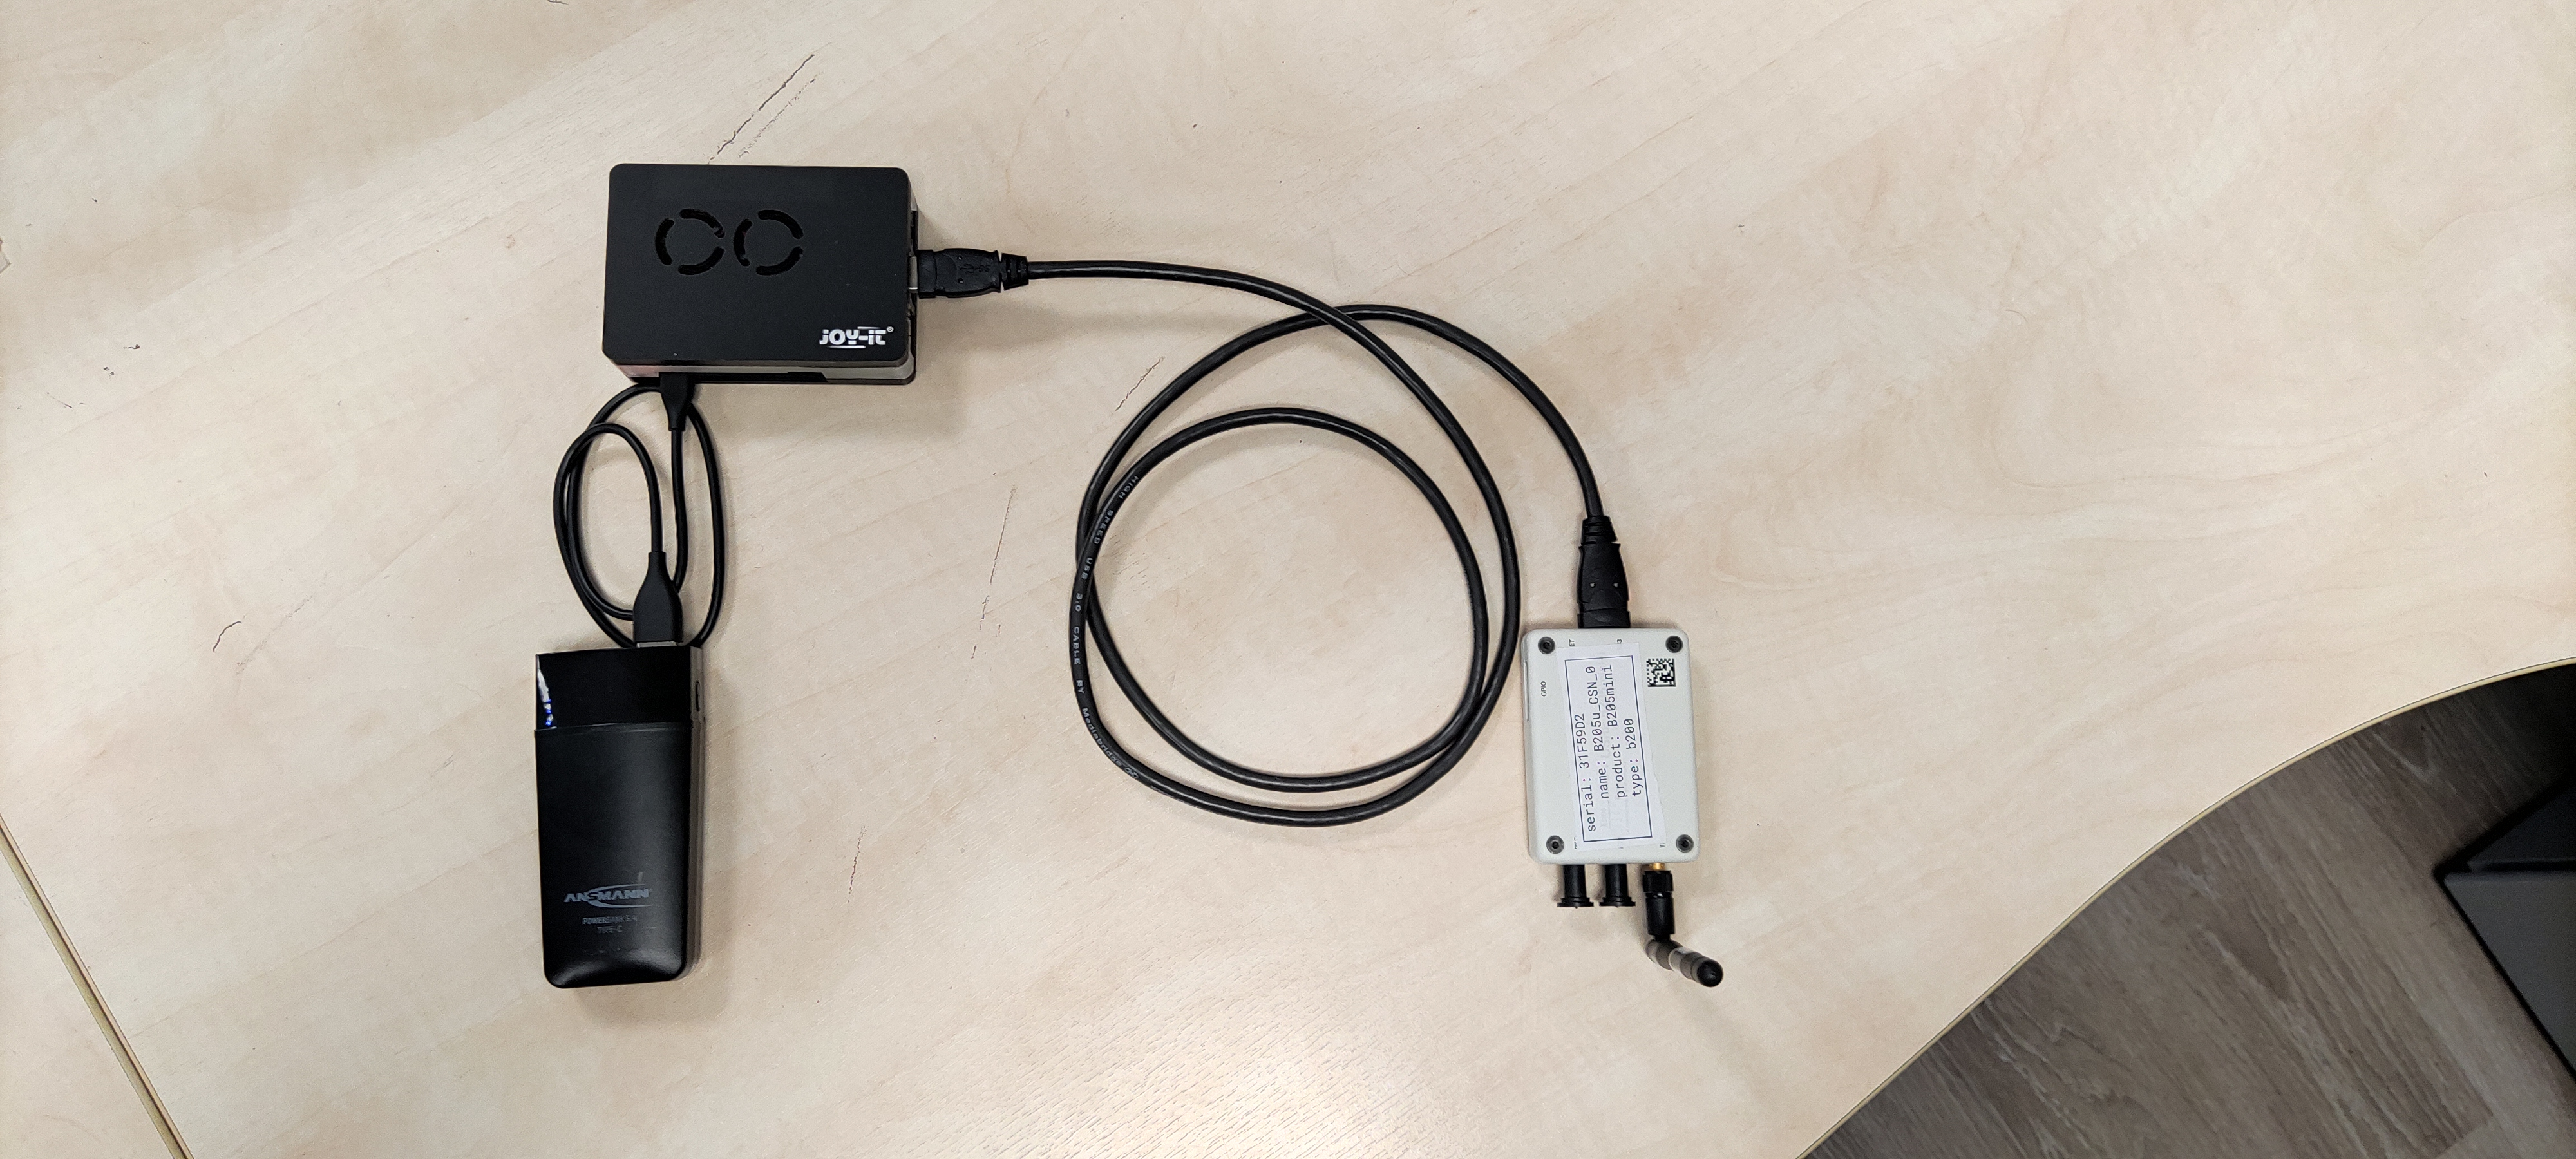
\includegraphics[height = .25\textheight, clip, trim = {800px 200px 1200px 200px}]{rtexps-pics/IMG_20221027_172657.jpg}
          \captionof{figure}{Émetteur autonome\\Raspberry Pi~4 et ``B205 mini'' alimentés par batterie.}
        \end{column}
        \begin{column}{.5\linewidth}
          \centering
          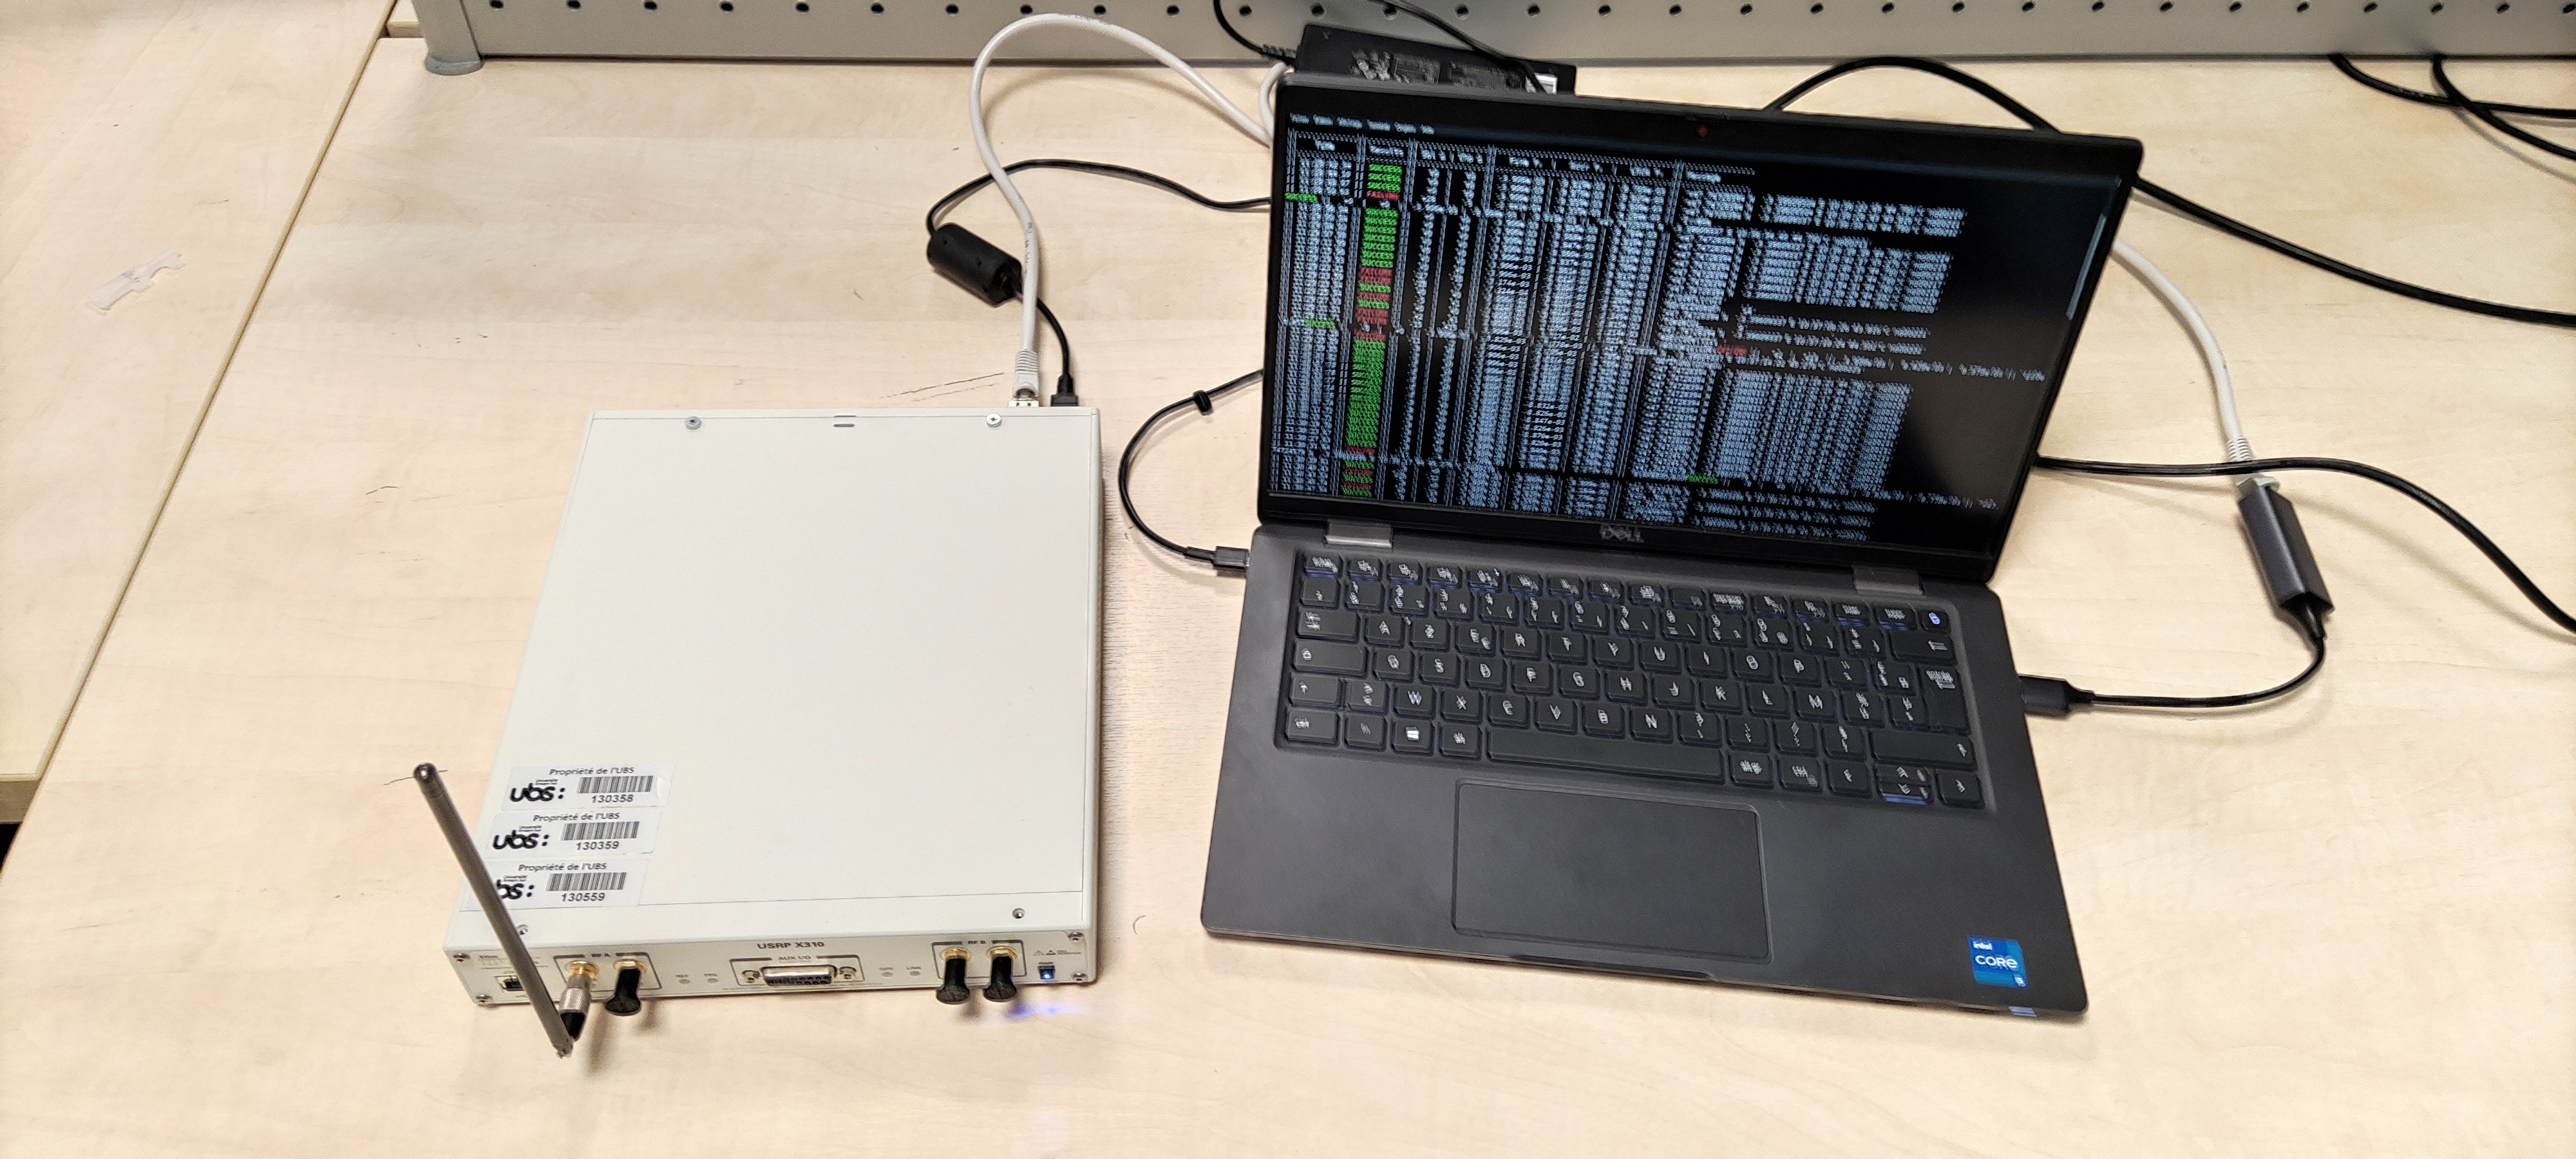
\includegraphics[height = .25\textheight, clip, trim = {600px 100px 600px 100px}]{rtexps-pics/IMG_20221027_180621.jpg}
          \captionof{figure}{Récepteur temps réel\\``X310'' et Ordinateur portable branché sur le secteur.}
        \end{column}
      \end{columns}
    \end{column}
  \end{columns}

  \vspace{1 em}

  \begin{columns}
    \begin{column}{.95\linewidth}
      \includegraphics[height = .18\textheight]{tikzpicture/transmission_demo_stdl.pdf} \hfill \vspace{.5 em} \\
      \hfill 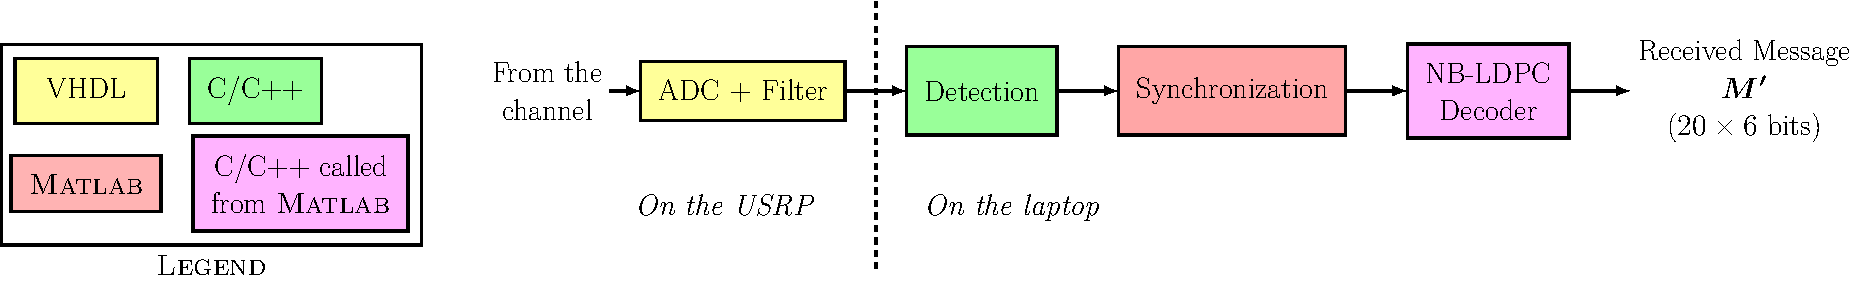
\includegraphics[height = .2\textheight]{tikzpicture/receiver_demo_stdl.pdf}
    \end{column}
  \end{columns}
  \note{
    \begin{enumerate}
      \item Objectif : validation de l'algo et du temps réel.
      \item Long travail d'ingénierie, rarement valorisable scientifiquement MAIS important.
      \item Donc -> travail d'equipe, \textbf{J'AI} rassemblé les bloc etc -> chronophage.
      \item MAIS DEMONSTRATEUR TEMPS RÉEL
    \end{enumerate}
  }
\end{frame}

\subsection{En ville}

\begin{frame}{\subsecname}
  \begin{columns}
    \begin{column}{.5\linewidth}
      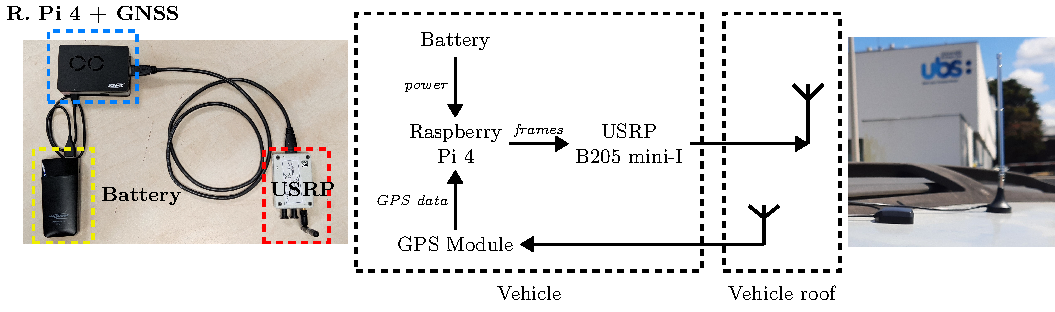
\includegraphics[height=.275\textheight]{tikzpicture/transmitter_sch_stdl.pdf}
      \captionof{figure}{Schéma du transmetteur QCSP itinérant}
    \end{column}
    \begin{column}{.5\linewidth}
      \begin{overlayarea}{\linewidth}{.55\textheight}
        \begin{itemize}
          \item Émission d'une trame toutes les $5$ secondes ;
          \item Débit de $500$ ks/s ($= 125$ kc/s) ;
          \item Émission en bande ISM ;
          \item Contenu de la trame : position GPS, compteur de trames, temps d'envoi et température du SoC.
        \end{itemize}
      \end{overlayarea}
    \end{column}
  \end{columns}

  \begin{columns}
    \begin{column}{.3\linewidth}
      \begin{itemize}
        \item Émetteur disposé dans une voiture, mobile ;
        \item Récepteur disposé en hauteur, fixe.
      \end{itemize}
    \end{column}
    \begin{column}{.7\linewidth}
      \includegraphics[height=.25\textheight]{tikzpicture/receiver_sch_stdl.pdf}
      \captionof{figure}{Schéma du récepteur QCSP fixe}
    \end{column}
  \end{columns}
\end{frame}

\begin{frame}
  \frametitle{Résultats}
  \begin{columns}
    \begin{column}{.5\linewidth}
      \hfill 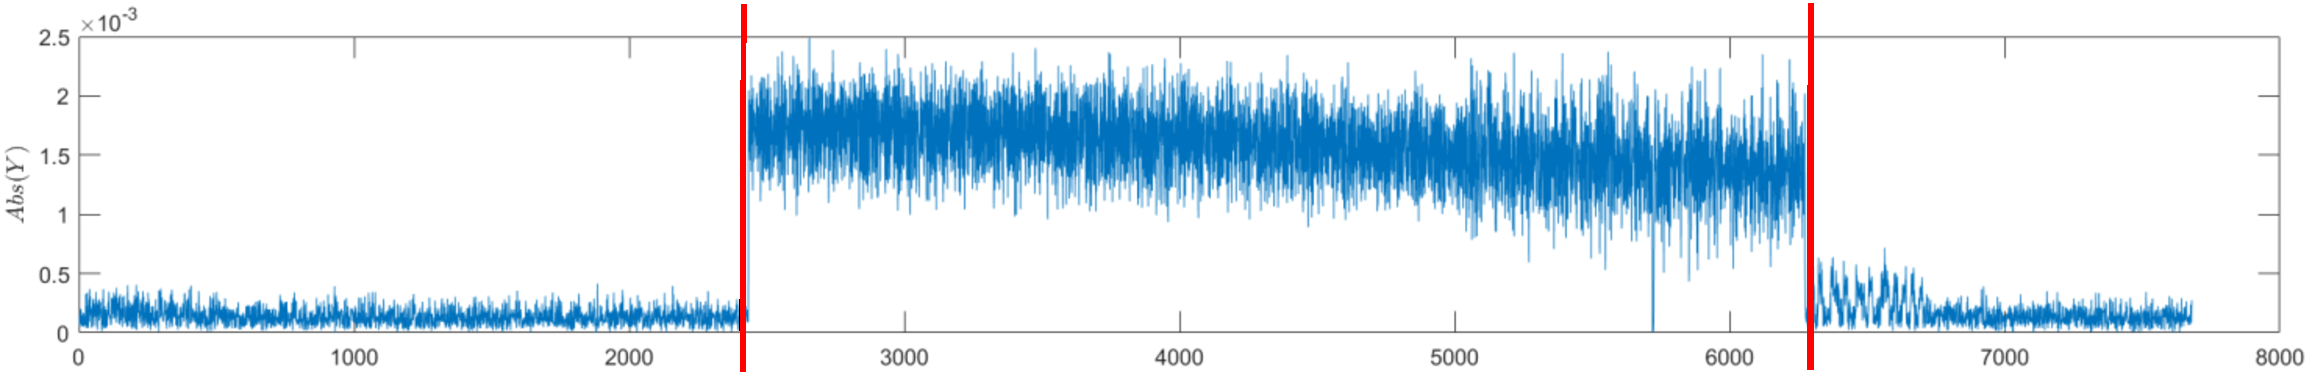
\includegraphics[width = .9\linewidth]{frame_high_snr_mark.pdf} \vspace{.5 em} \\
      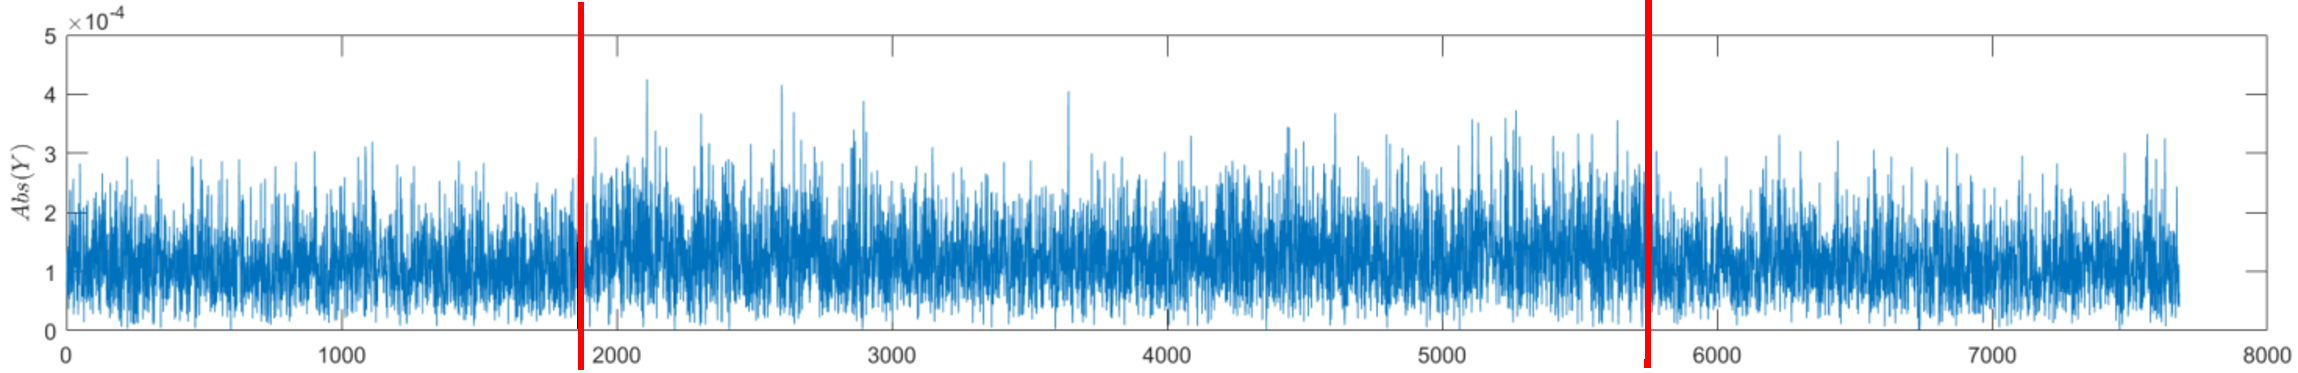
\includegraphics[width = .9\linewidth]{frame_low_mark.pdf} \vspace{.5 em} \\
      \hfill 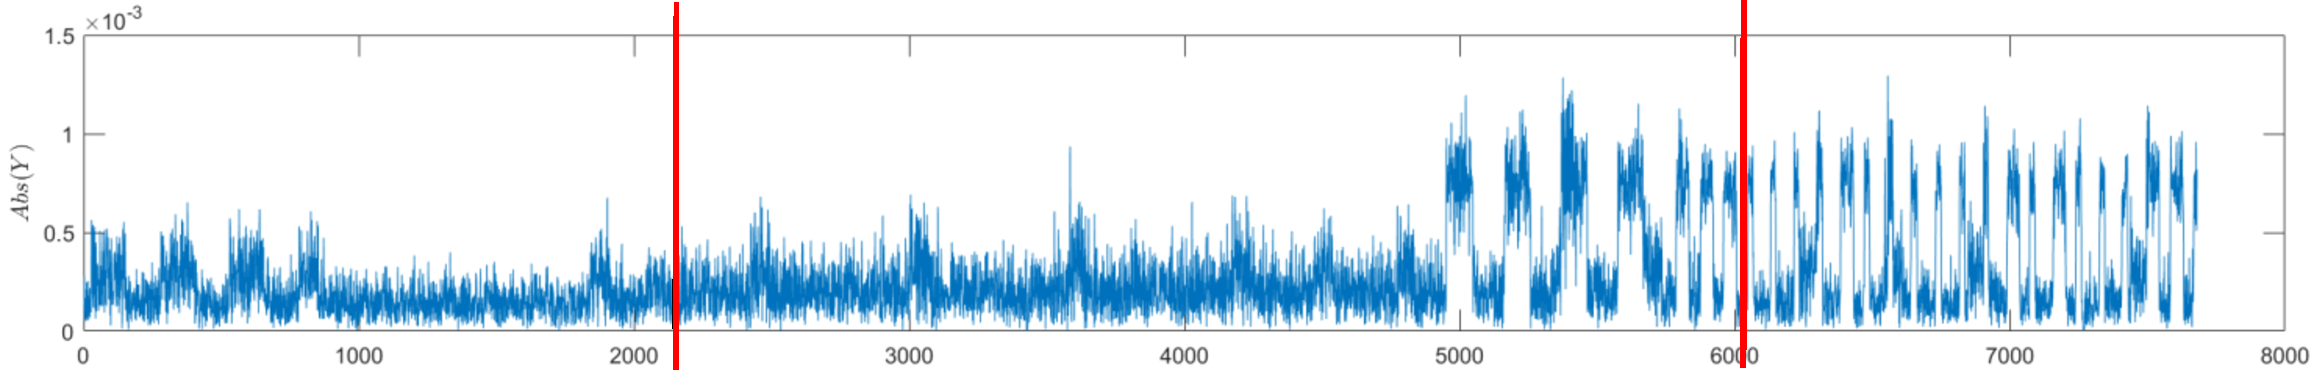
\includegraphics[width = .9\linewidth]{frame_low_interf_mark.pdf} \vspace{.5 em} \\
      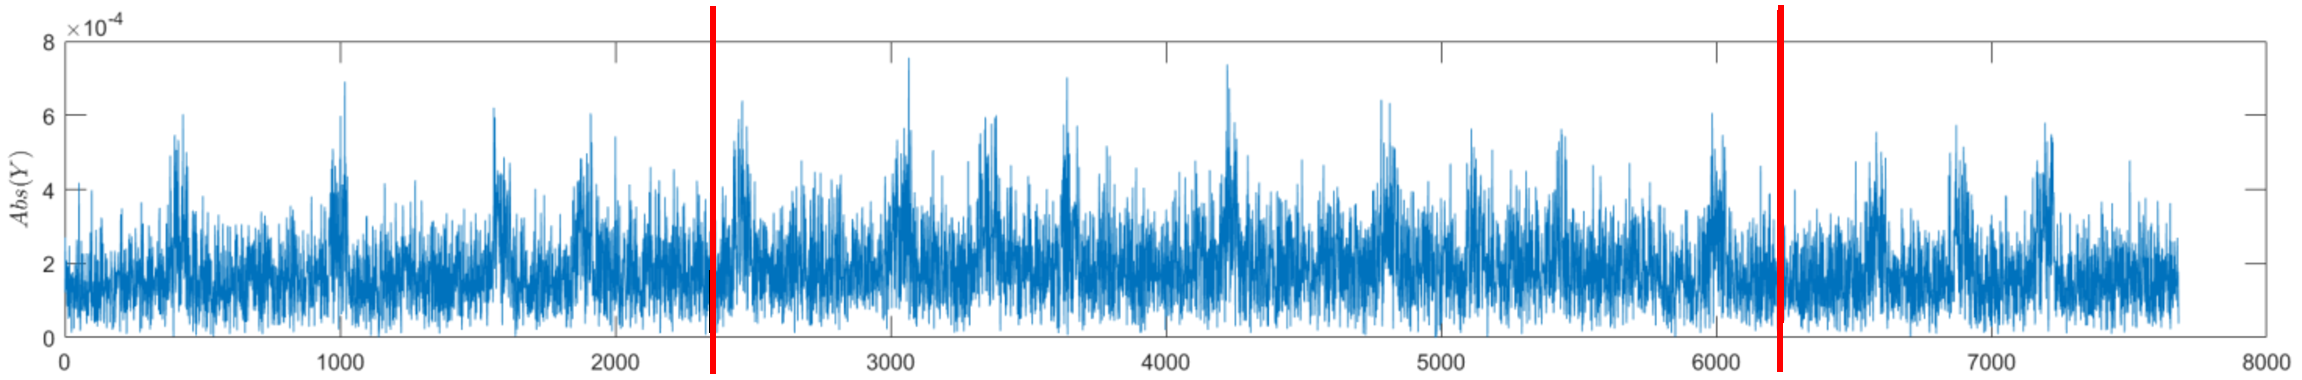
\includegraphics[width = .9\linewidth]{frame_low_interf2_mark.pdf}
      \captionof{figure}{Données brutes du canal correspondant à $4$ trames reçues et décodées avec succès.}
    \end{column}
    \begin{column}{.5\linewidth}
      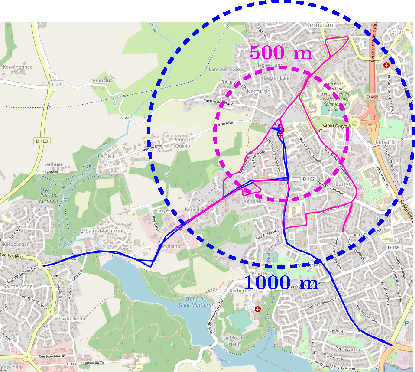
\includegraphics[width = .9\linewidth]{tikzpicture/gpx_track_rex_stdl.pdf}
      \captionof{figure}{Portée maximale pour deux campagne de données --- Les antennes utilisées pour la \textcolor{Blue}{$1$ère en bleu} était mieux adapté que pour la \textcolor{Magenta}{$2$nd en magenta}.}
    \end{column}
  \end{columns}
\end{frame}

\subsection{En mer}

\begin{frame}{\subsecname}
  \begin{columns}
    \begin{column}{.5\linewidth}
      \hfill 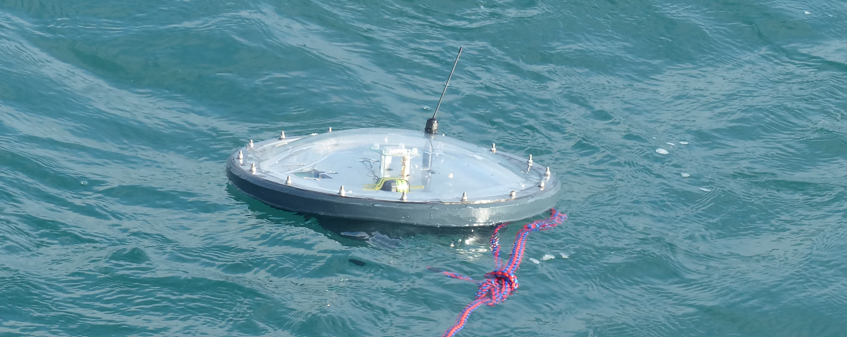
\includegraphics[width =\linewidth]{buoys_emitter.png}
    \end{column}
    \begin{column}{.5\linewidth}
      \begin{itemize}
        \item L'émetteur est embarqué dans une bouée autonome et transmet comme précédemment ;
      \end{itemize}
    \end{column}
  \end{columns}
  \begin{columns}
    \begin{column}{.5\linewidth}
      \begin{itemize}
        \item Le récepteur est embarqué dans un bateau qui se déplace autour de la zone de la bouée ;
        \item Analyse des résultats en cours \dots
      \end{itemize}
    \end{column}
    \begin{column}{.5\linewidth}
      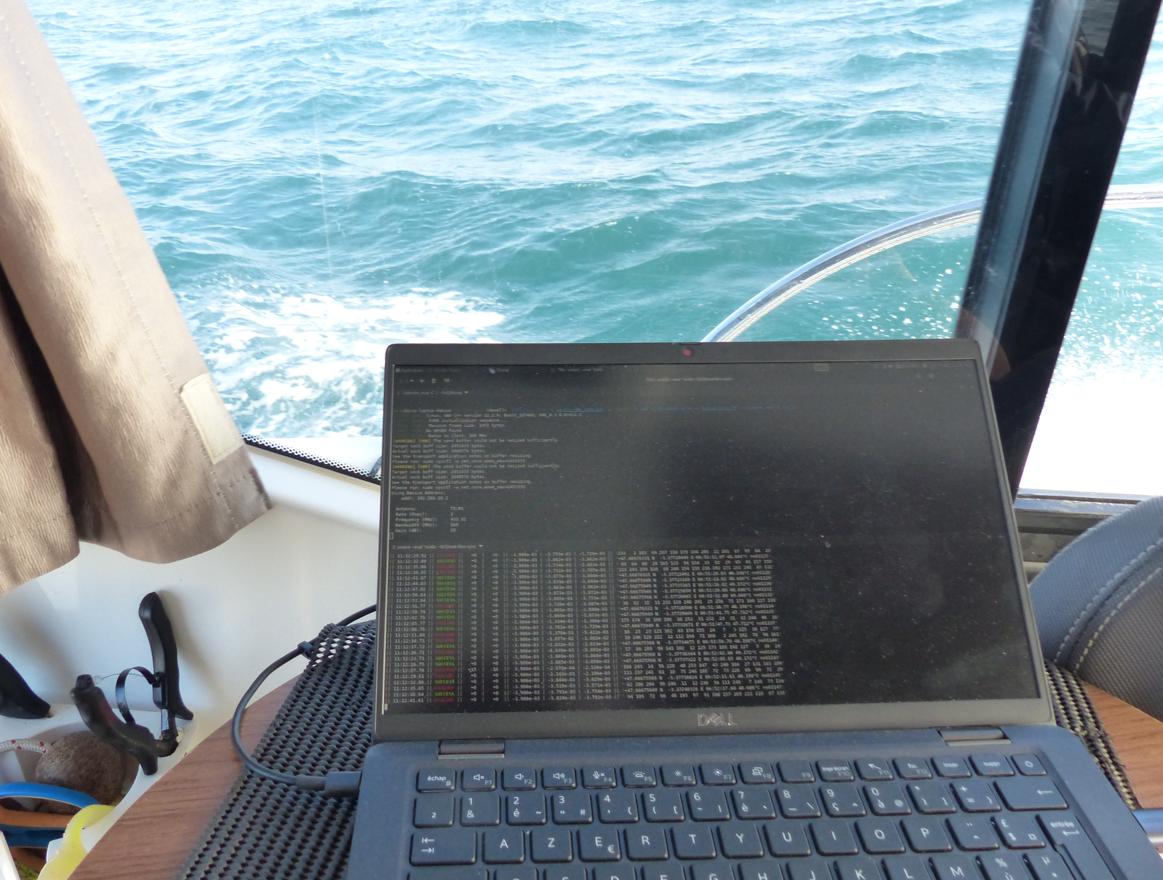
\includegraphics[height = .5\textheight, clip, trim = {200px 0 0 300px}]{boat_detector.png} \hfill
    \end{column}
  \end{columns}
  \note{
    C'est cool MAIS EN PLUS

    C'est pas moi qui ai fait -> la transmission est assurée.
  }
\end{frame}

\end{document}
